\documentclass{beamer} % Document class

\usepackage[english]{babel} % Set language
\usepackage[utf8x]{inputenc} % Set encoding

% 加入 listings 套件
\usepackage{listings}
\usepackage{xcolor}

% 設定 listings 樣式
\lstset{
    language=R,
    basicstyle=\ttfamily\small,
    backgroundcolor=\color{gray!10},
    frame=single,
    breaklines=true,
    showstringspaces=false,
    keywordstyle=\color{blue},
    commentstyle=\color{green!50!black},
    stringstyle=\color{red},
    numbers=none,
    xleftmargin=10pt,
    xrightmargin=10pt,
    framexleftmargin=5pt,
    framexrightmargin=5pt
}

\mode<presentation> % Set options
{
  \usetheme{default} % Set theme
  \usecolortheme{default} % Set colors
  \usefonttheme{default} % Set font theme
  \setbeamertemplate{caption}[numbered] % Set caption to be numbered
}

\usepackage{graphicx} % For including figures
\graphicspath{{figure/}} % Shared figure folder for all labs
\usepackage{booktabs} % For table rules
\usepackage{hyperref} % For cross-referencing
\usepackage{subcaption} % 記得加在 preamble
\usepackage{multicol}

\title{R Basic} % Presentation title
\author{Rex Shao-Yu Wang} % Presentation author
\institute{} % Author affiliation
\date{September 21, 2026} % Today's date

\begin{document}

% Title page
\begin{frame}
  \titlepage
\end{frame}

% Outline
\begin{frame}{Outline}
  \tableofcontents
\end{frame}

\section{Functions}
\begin{frame}{Functions}
    \begin{itemize}
        \item The building blocks of R programming. 
        \item Allow you to encapsulate a set of instructions and reuse them throughout your code.
        \item Can take inputs (arguments) and return outputs (results).
    \end{itemize}
    \begin{figure}
        \centering
        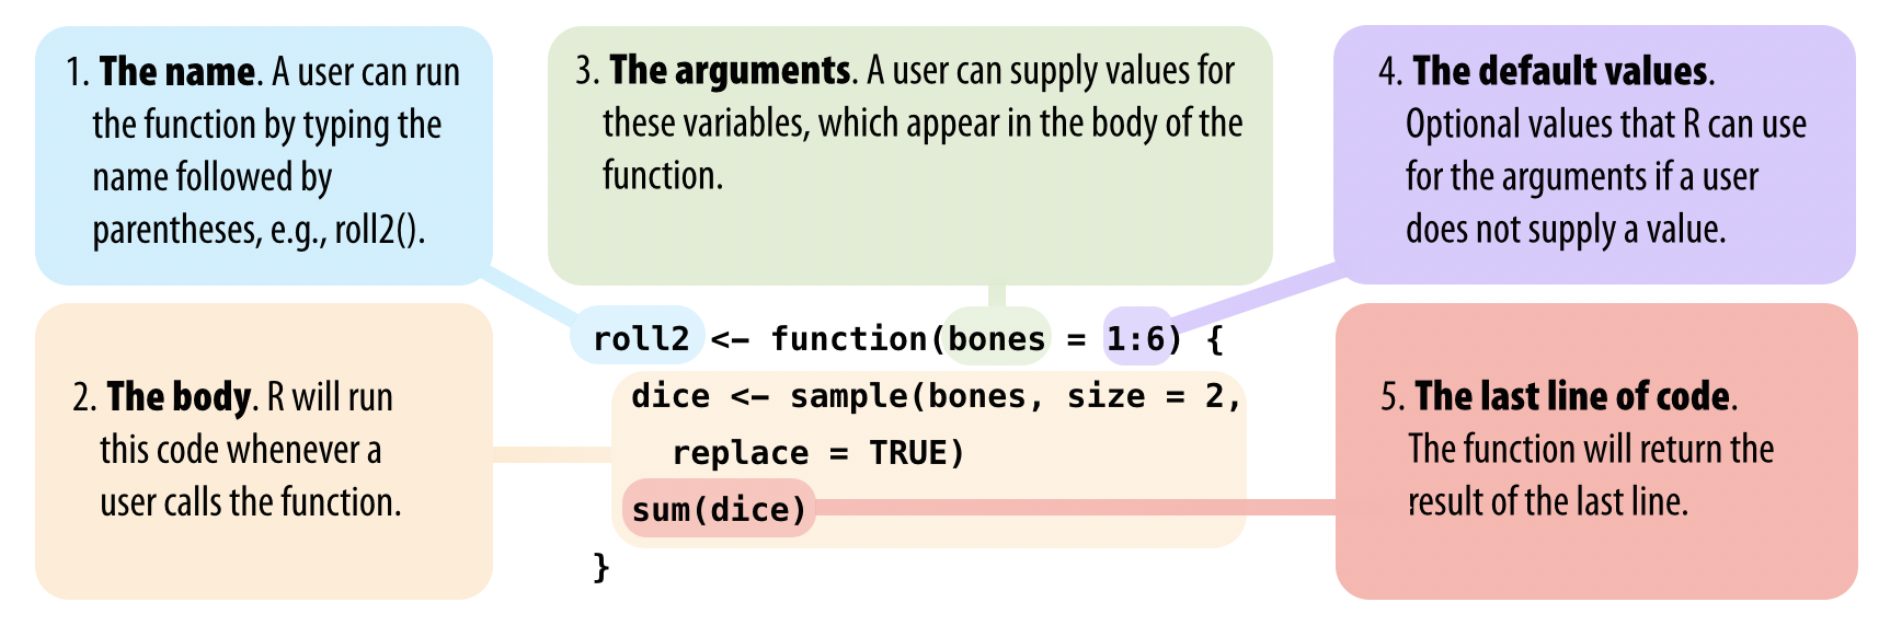
\includegraphics[width=1.05\linewidth]{functions.png}
    \end{figure}
\end{frame}

\begin{frame}[fragile]{Basic Built-in Functions in R}
    \begin{itemize}
        \item \texttt{round()}: Round a number to a specified number of decimal.
        \item \texttt{factorial()}: Calculate the factorial of an integer (non-neg.).
        \item \texttt{sum()}: Calculate the sum of a set of numbers.
        \item \texttt{mean()}: Calculate the average of a set of numbers.
        \item \texttt{sample()}: Randomly select a specified number of elements from a set of numbers.
    \end{itemize}
    \begin{lstlisting}
round(3.14159, digits = 2) # Output: 3.14
factorial(5) # Output: 120
sum(1:6) # Output: 21
mean(1:6) # Output: 3.5

# sample without replacement
sample(1:10, size = 3, replace = FALSE) 

# sample with replacement
sample(1:10, size = 3, replace = TRUE) 
    \end{lstlisting}
\end{frame}

\begin{frame}[fragile]{Create your own function} 
    You're rolling pairs of dices, and you want to calculate the sum of the two dices. \\
    You can create a function to do this:
    \begin{lstlisting}
roll_dice <- function() {
    die <- sample(1:6, size = 2, replace = TRUE)
    sum(die)
}

# Call the function to roll the dice and get the sum
roll_dice() 
    \end{lstlisting}
\end{frame}

\section{Data Structure} 

\begin{frame}{Basic Data Structure}
  \begin{tabular}{ll}
    \toprule
    \textbf{Type} & \textbf{Range}                                          \\
    \midrule
    Vector       & A list of items that are of the same type                \\
    Matrix       & A two-dimensional data set with columns and rows         \\
    List         & A collection of items that can be of different types     \\
    Data frame   & Data displayed in a format as a table                    \\
    \bottomrule
  \end{tabular}

  \begin{figure}
    \centering
    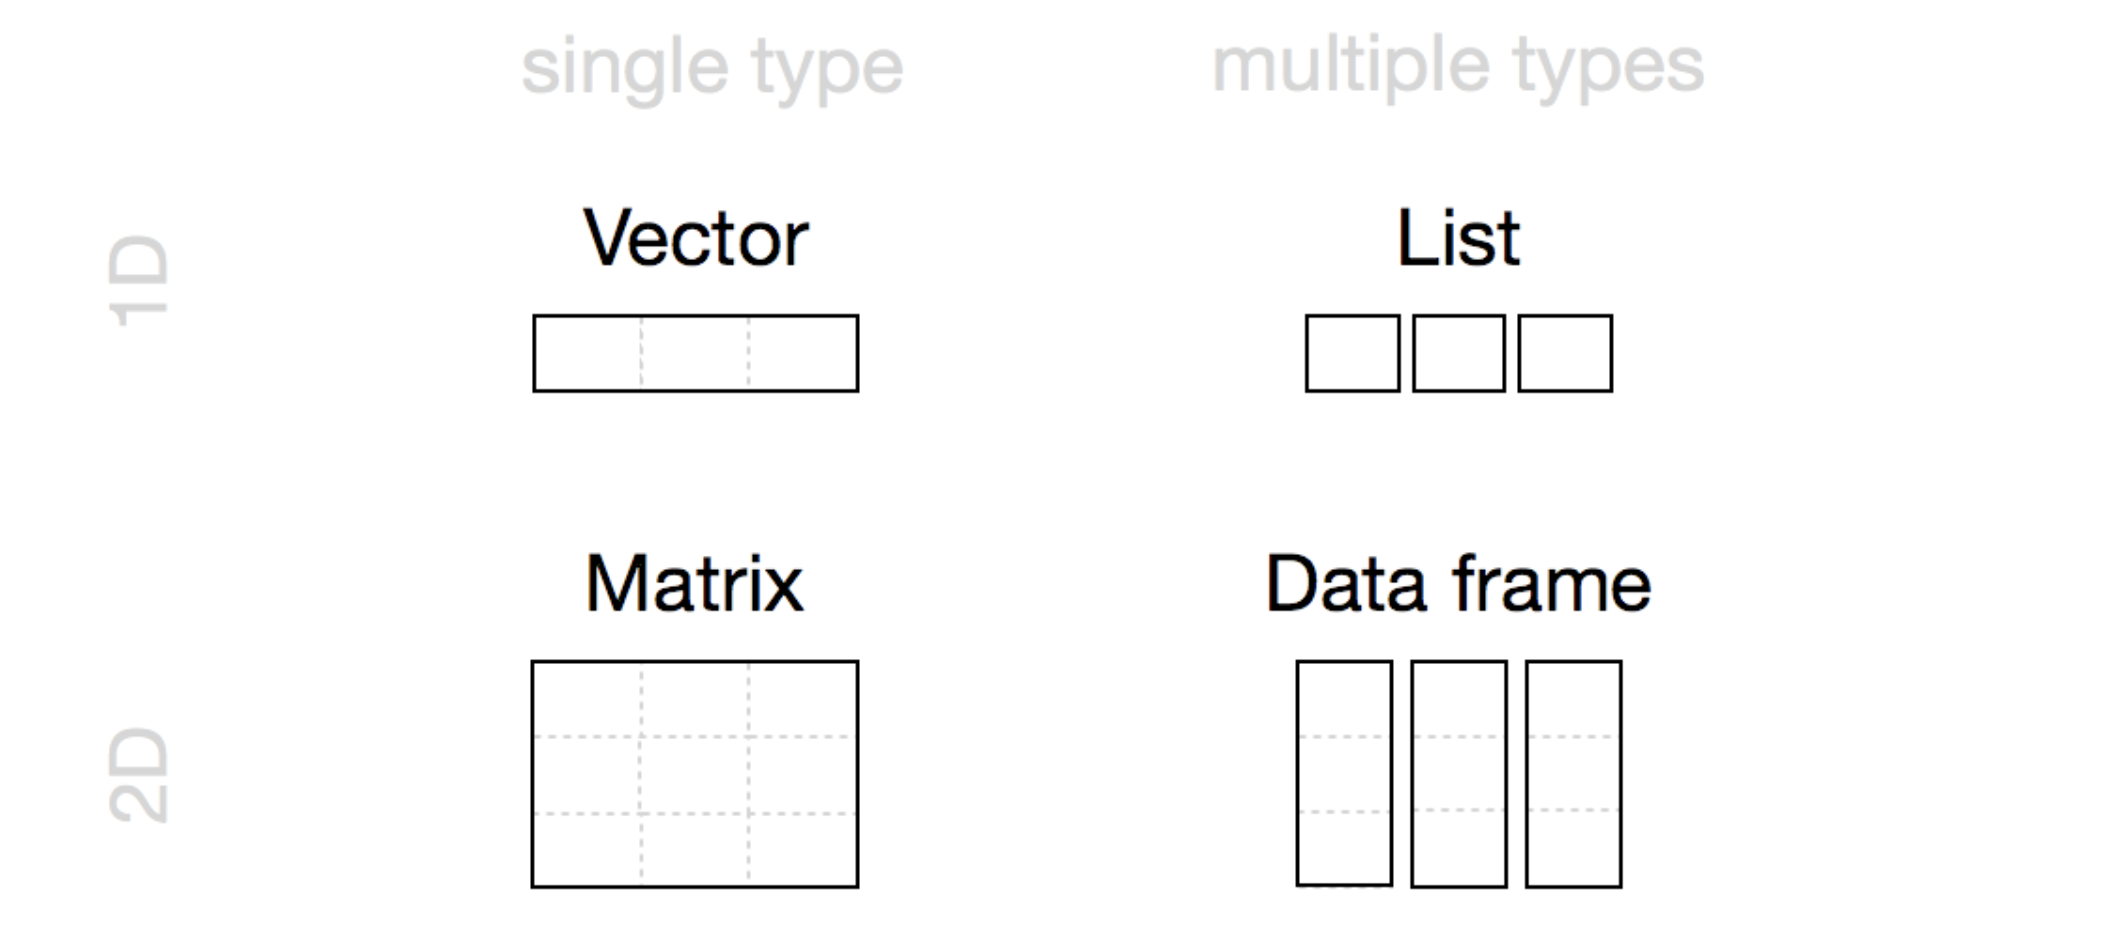
\includegraphics[width=0.9\linewidth]{data_structure.png}
  \end{figure}
\end{frame}

\subsection{Atomic Vectors}
\begin{frame}{Atomic Vectors} 
    A simple data type that contains elements of the same type. \\
  \begin{tabular}{lll} 
    \toprule
    \textbf{Type} & \textbf{Store}      & \textbf{Assign a Value}               \\
    \midrule
    Doubles      & Regular numbers     & \texttt{die <- c(1, 2, 3, 4, 5, 6)}    \\
    Integer      & Integers            & \texttt{int <- c(-1L, 2L, 4L)}         \\
    Character    & Text strings        & \texttt{text <- ("Hello", "World")}    \\
    Logical      & TRUE or FALSE       & \texttt{logic <- c(TRUE, FALSE, T)}    \\
    Complex      & Complex numbers     & \texttt{comp <- c(1 + 1i, 1 + 2i)}     \\
    \bottomrule
  \end{tabular} \\
  \vspace{20pt}
  \texttt{typeof()}: To check what type of obeject you are working \\
  \texttt{length()}: To check how many elements are in the vector
\end{frame}

\begin{frame}[fragile]{Vectors}  
  \texttt{c()} stands for concatenate, which combines elements into a vector
  \begin{lstlisting}
die <- c(1, 2, 3, 4, 5, 6)
text <- ("Hello", "World")
  \end{lstlisting}

  \texttt{rep()}: Replicate elements of vectors and lists
  \begin{lstlisting}
rep(x = 1, times = 9)
rep(x = c(1, 2), each = 3)
rep(x = c(1, 2, 3), times = c(2, 3, 5))
  \end{lstlisting}

  \texttt{seq()}: Tool used to generate regular sequences of numbers
  \begin{lstlisting}
seq(from = 1, to = 5, by = 1)
seq(1, 9, by = 2)
seq(0, 1, length.out = 11)
  \end{lstlisting}
\end{frame}

\subsection{Matrices}
\begin{frame}[fragile]{Matrices}
  \begin{columns}
    \column{0.72\textwidth}
    Matrices store values in a two-dimensional array. \\
    \vspace{10pt}
    How to create a matrix in R? \\
    \texttt{matrix(data, nrow, ncol, byrow)} 
    \begin{itemize}
      \item data: give it a vector of values
      \item nrow: specifies the number of rows
      \item ncol: specifies the number of columns
      \item byrow: fill the matrix by row or by column
    \end{itemize}
    \begin{lstlisting}
die <- c(1, 2, 3, 4, 5, 6)
matrix(data = die, nrow = 2, ncol = 3, byrow = T)
matrix(data = die, nrow = 2, byrow = F)

die.mx <- matrix(die, nrow = 2)
    \end{lstlisting}

    \column{0.4\textwidth}
    \vspace{0pt}
    \begin{figure}
      \centering
      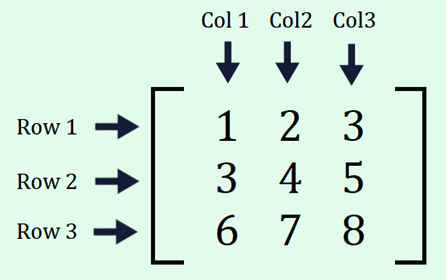
\includegraphics[width=1\linewidth]{截圖 2026-03-07 上午10.14.08.png}
    \end{figure}

    Check the structure with
    \begin{lstlisting}
dim(die.mx)
length(die.mx)
nrow(die.mx)
ncol(die.mx)
    \end{lstlisting}
  \end{columns}
\end{frame}

\begin{frame}[fragile]{Data Frames}
  \texttt{data.frame()} creates data frames, coupled collections of variables
  \begin{columns}
    \column{0.55\textwidth}
    \begin{lstlisting}
information <- data.frame(
  Name = name,
  Class = class,
  Score = score
)
    \end{lstlisting}

    \column{0.45\textwidth}
    \begin{figure}
      \centering
      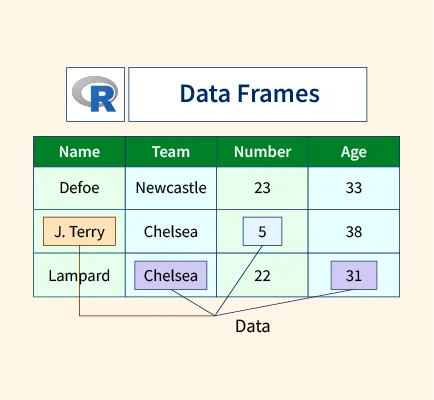
\includegraphics[width=1.1\linewidth]{data-frames-in-r-thumbnail.png}
    \end{figure}
  \end{columns}
\end{frame}

\subsection{Lists}
\begin{frame}[fragile]{Lists}
  jjj
\end{frame}

\subsection{Data Frame}
\begin{frame}[fragile]{Data Frame}
  \begin{columns}
    \column{0.55\textwidth}
    What will these commands do?
    \begin{lstlisting}
information["Name"]
information[2]
information[2, ]
information[1:3]
information$Name
    \end{lstlisting}
    Check the structure with
    \begin{lstlisting}
colnames(information)
rownames(information)
length(information)
nrow(information)
ncol(information)
    \end{lstlisting}

    \column{0.45\textwidth}
    \begin{figure}
      \centering
      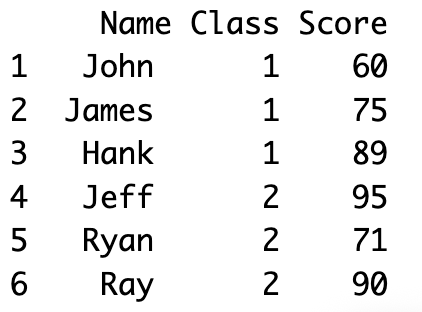
\includegraphics[width=1.1\linewidth]{截圖 2026-03-09 上午10.16.03.png}
    \end{figure}
  \end{columns}
\end{frame}

\section{R Notation}
\subsection{Selecting Values}
\begin{frame}[fragile]{Selecting Values}
  What will these commands do?
  \begin{lstlisting}
score[1]
score[1:3]
score[c(1, 2, 5)]
  \end{lstlisting}
  \begin{figure}
    \centering
    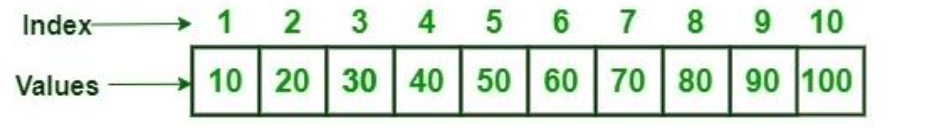
\includegraphics[width=0.7\linewidth]{截圖 2026-03-07 凌晨2.20.14.png}
  \end{figure}

  \begin{columns}
    \column{0.55\textwidth}
    What will these commands do?
    \begin{lstlisting}
die.mx[1]
die.mx[1, 2]
die.mx[, c(1, 3)]
    \end{lstlisting}

    \column{0.45\textwidth}
    \begin{figure}
      \centering
      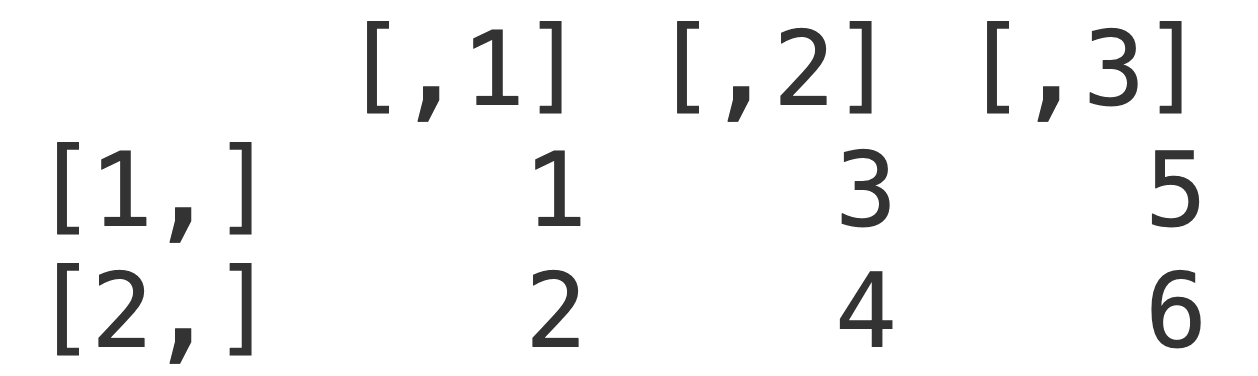
\includegraphics[width=1\linewidth]{matrix_example.png}
    \end{figure}
  \end{columns}
\end{frame}

\begin{frame}[fragile]{Dollar Signs and Double Brackets}
  fff
\end{frame}
\subsection{Modifying Values}
\begin{frame}[fragile]{Modifying Values}
  fff
\end{frame}



\section{Lab Report}
\begin{frame}{Lab Report}
  \begin{itemize}
    \item The report file will be in the NTU COOL Assignment section
    \item Submit your file in pdf format
    \item Deadline: 10/5 (Mon) 13:20 (Before the next class started)
    \item Late submission is not accepted
  \end{itemize}
\end{frame}

\begin{frame}[fragile]{Exercises: Vectors in R}
  \begin{enumerate}
    \item Use the seq() function to generate the sequence \\  9, 18, 27, 36, 45.
    \item Use the rep() function to generate the sequence \\ 1 1 1 1 1 2 2 2 2 3 3 3 4 4 5
    \item Given the following vectors:
    \begin{lstlisting}
students <- c("Alice", "Bob", "Chris", "David", "Eve")
    \end{lstlisting}
    Write the R commands to:
    \begin{enumerate}
      \item Extract the first element from the \texttt{students} vector.
      \item Extract the first three elements from the \texttt{students} vector.
      \item Extract all names from \texttt{students} \textbf{except} for the second one ("Bob").
    \end{enumerate}
  \end{enumerate}
\end{frame}
\end{document}
